\documentclass{hw}

\usepackage{tikz}
\usetikzlibrary{automata,positioning}

\begin{document}
\section*{Stochastic Modeling}

A stochastic matrix is a square matrix whose elements are probabilities and where each row sums to
one. One special example of a stochastic matrix is a matrix of transition probabilities.

\begin{quote}
\textit{\textbf{Example}}\\
Consider the case where a student enters a college as a one major, but changes to another.

\begin{center}
\begin{tabular}{c | c c c}
& STEM & Humanities & Business\\
\hline
STEM & 0.6 & 0.3 & 0.1\\
Hum. & 0.05 & 0.7 & 0.25\\
Bus. & 0.2 & 0.3 & 0.5
\end{tabular}
\end{center}

In this matrix, each $a_{ij}$ entry represents the probability that a student will change to that
major (or keep that major if it is the same). Suppose we have 1000 freshmen that enter the college
\[
x_{0}=[300,500,200]
\]
in the order STEM, Humanities, and Business. If we want to know the number of STEM majors in the
class's sophomore year, we can multiply our initial vector by the STEM column of our matrix:
\begin{align*}
\text{STEM Majors}&=(0.6)(300)+(0.05)(500)+(0.2)(200)\\
&=245\text{ students}\\
\text{Hum. Majors}&=(0.3)(300) + (0.7)(500) + (0.3)(200)\\
&= 500\text{ students}\\
\text{Bus. Majors}&=(0.1)(300) + (0.25)(500) + (0.5)(200)\\
&=255\text{ students}
\end{align*}
We can continue this process for each year that the students attend the college.
\end{quote}

This process for creating a sequence of vectors is called a Markov Chain. In general, we can
start with a vector $\bf{x}_{0}$ and a matrix $P$, and we get that
\begin{alignat*}{3}
\bf{x}_{1}&=\bf{x}_{0}\cdot P\\
\bf{x}_{2}&=\bf{x}_{1}\cdot P &&= \bf{x}_{0}\cdot P\cdot P\\
\bf{x}_{3}&=\bf{x}_{2}\cdot P &&= \bf{x}_{0}\cdot P\cdot P\cdot P,\\
\end{alignat*}
which yields the recurrence relation
\[
\bf{x}_{n}=\bf{x}_{0}P^{n}.
\]
$P^{n}$ is called the $n$-step transition matrix. In this matrix, the $a_{ij}$ element gives the
probability of going from state $i$ to state $j$.

\begin{quote}
\textit{\textbf{Example}}\\
Consider the movement of people from the city to the suburb.
\begin{center}
\begin{tabular}{c | c c}
& Cities & Suburbs\\
\hline
Cities & 0.96 & 0.04\\
Suburbs & 0.1 & 0.99
\end{tabular}
\end{center}
with the initial vector
\[
\bf{x}_{0}=[60,125].
\]
We can introduce some ``noise" into the system by discussing the eigenvalues of this system. In the
usual case, $\lambda=1$. We can show this by solving the system.
\begin{align*}
(\bf{P}-\lambda)\bf{x}&\to
\left[
\begin{array}{c c c}
-0.4 & 0.4 & 0\\
0.1 & 0.1 & 0
\end{array}
\right]\\
&\to
\left[
\begin{array}{c c c}
1 & -1 & 0\\
0 & 0  & 0
\end{array}
\right],
\end{align*}
so $x=y=1$.
\end{quote}

Often in Markov processes, we come across matrices raised to a power. To help us calculate these
products, we can come up with a new matrix, $\bf{S}$. We can then calculate
$\bf{S}^{-1}\bf{D}\bf{S}$, where $D$ is diagonalized matrix of the eigenvalues of $\bf{P}$. We know
that we can diagonalize $\bf{P}$ by the following theorem:
\begin{quote}
An $n\times n$ matrix $\bf{P}$ is diagonalizable if and only if it has $n$ linearly independent
eigenvectors.\\\\

\textit{\textbf{Example}}\\
Consider three types of detergent that yield the Markov matrix
\begin{center}
\begin{tabular}{c | c c c}
& Tide & Bounty & Bounce\\
\hline
Tide & .8 & .1 & .1\\
Bounty & .2 & .6 & .2\\
Bounce & .3 & .3 & .4
\end{tabular}
\end{center}
where the entries indicate the probability that a user will stay with that product. Rather than
finding the next state, we will consider a vector $\pmb{\pi}$, called the limiting state probability
vector. This vector will be representative of the probabilities of users staying with a brand.
Similar to the previous examples, we have
\[\pmb{\pi}\bf{P}=\pmb{\pi}.\]
From this equation, we get
\[
\begin{cases}
.8\pi_{1}+.2\pi_{2}+.3\pi_{3}=\pi_{1}\\
.1\pi_{1}+.6\pi_{2}+.3\pi_{3}=\pi_{2}\\
.1\pi_{1}+.2\pi_{2}+.4\pi_{3}=\pi_{3}
\end{cases}
\]
The third equation in this case is a linear combination of the first two, so we cannot user it here.
However, we can replace it with a linearly independent row:
\[
\begin{cases}
.8\pi_{1}+.2\pi_{2}+.3\pi_{3}=\pi_{1}\\
.1\pi_{1}+.6\pi_{2}+.3\pi_{3}=\pi_{2}\\
\pi_{1}+\pi_{2}+\pi_{3}=1
\end{cases}
\to
\left[
\begin{array}{c c c | c}
-.2 & .2 & .3 & 0\\
.1 & -.4 & .3 & 0\\
1 & 1 & 1 & 0
\end{array}
\right]
\to
\pmb{\pi}=
\left[
\begin{array}{c}
{6/11}\\
{3/11}\\
{2/11}
\end{array}
\right].
\]
\end{quote}

\section*{Irreducible Matrices}
We attempted to find the $\pi$ vector in the previous examples. We can use the following theorem to
discuss special Markov Chains.
\begin{quote}
Let $P$ be the transition matrix for an irreducible and aperiodic Markov Chain. Then there exists
a unique probability vector $\pi$ such that
\[
\pi\cdot P=\pi.
\]
\end{quote}
It follows that if $P$ is a regular matrix, then we can also find the $\pi$ vector. A more
interesting phenomenon occurs when we do not have a regular $P$ matrix. A typical model of this can
be seen in the Drunkard's walk without reflection.

\subsection*{The Drunkard's Walk}
The Drunkard's walk represents a random walk with several states. At some states, the drunk man may
either end up in his bed or on the street. In the reflective version of this walk, it is possible that
after going into his bed, the drunkard goes back out. In this example, we want to consider absorbing
states, which are states that are not able to be escaped.

In this walk, we want to model the drunkard by saying that if he falls asleep in the street or he
goes to his bed, then the walk ends. Those conditions are representative of absorbing states.
\[
P=
\left(
\begin{array}{c c c c c}
1 & 0 & 0 & 0 & 0\\
1/2 & 0 & 1/2 & 0 & 0\\
0 & 1/2 & 0 & 1/2 & 0\\
0 & 0 & 1/2 & 0 & 1/2\\
0 & 0 & 0 & 0 & 1
\end{array}
\right).
\]
More generally, an absorbing matrix takes the form of an $r\times r$ matrix with $k$ absorbing
states. It is a fact that ultimately everything will end up in the absorbed state. Markov Chains
are only absorbing when all absorbing state can be reached. If a state is not absorbing, it is
called a transient state.

For the drunkard's walk, we can partition the matrix into four parts:
\[
P=
\left(
\begin{array}{c c c c c}
1 & 0 & 0 & 0 & 0\\
1/2 & 0 & 1/2 & 0 & 0\\
0 & 1/2 & 0 & 1/2 & 0\\
0 & 0 & 1/2 & 0 & 1/2\\
0 & 1/2 & 0 & 1/2 & 0
\end{array}
\right)
=
\left(
\begin{array}{c c c c c}
1 & 0 & 0 & 0 & 0\\
0 & 1 & 0 & 0 & 0\\
1/2 & 0 & 0 & 1/2 & 0\\
0 & 0 & 1/2 & 0 & 1/2\\
0 & 0 & 0 & 0 & 1
\end{array}
\right)
\]
which allows us to calculate a new matrix $N=(I-Q)^{-1}$. Every $n_{ij}$ entry in the $N$ matrix
tells us the average number of times that the process is in the $j$ state if it starts in the $i$
state.

\section*{Poisson Probabilities}

Suppose that $f(x,t)$ is the probability of getting $x$ successes during a time interval of length
$t$. Assume the prob of success during a very small time internal from $t$ to $t+\delta t$ is $\mu$,
the probability of more than one success during a time interval is negligible, and the probability
of a success during such a time interval does not depend on what happened prior to time $t$. The
Poisson distribution is given by
\[
f(x,t+\Delta t)=f(x,t)\cdot[1-\mu\Delta t]+f(x-1,t)\mu\Delta t = {e^{-\mu}\mu^{x}\over x!}
\]
The variable $x$ is indicative of the number of successes we want in the next time interval
$t+\delta t$. One example of the use of Poisson distributions is to calculate the probability that
an earthquake will occur again in a certain area.\\\\

\begin{quote}
\textit{\textbf{Example}}\\
Suppose that in southern California, 5 earthquakes occur every 100 years on average. What is the
probability that 2 earthquakes will occur in the next century?\\\\

The answer is very straightforward:
\[
P={e^{-5}5^{2}\over 2!}
\]
If we wanted to know the probability in the next 10 years, we can calculate
\[
P={e^{-0.5}0.5^{2}\over 2!}.
\]
\end{quote}

\section*{Markov Chains and Continuity}
We can form a relationship between Markov Chains and differential equations.
\begin{quote}
\textit{\textbf{Example}}\\
In the summer, an AC unit is in one of 3 states: (0) off, (1) low, or (2) high. While off,
transitions to low occur after an exponential time with an expected time of 3 minutes.
\begin{center}
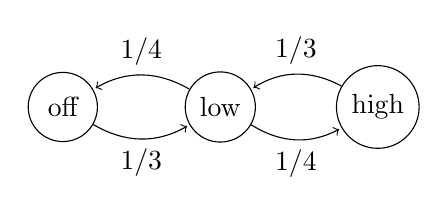
\begin{tikzpicture}[shorten >=1pt,node distance=2cm,on grid,auto]
    \node[state] (off) {off};
    \node[state] (low)[right=of off] {low};
    \node[state] (high)[right=of low] {high};
    \path[->]
    (off) edge[bend right,swap] node {$1/3$} (low)
    (low) edge[bend right,swap] node {$1/4$} (off)
          edge[bend right,swap] node {$1/4$} (high)
    (high) edge[bend right,swap] node {$1/3$} (low);
\end{tikzpicture}
\end{center}
We assign a $\lambda$ value to each state where $\lambda\in(0,\infty)$. The density function is
given by
\[
f(t)=\lambda e^{-\lambda t}
\]
for $t>0$. We can call the waiting time $T_{n}$, where $n$ is the state where we want to move. If
we have $T_{1}$ and $T_{2}$, the smaller $T$ is the state to which we move.
\end{quote}


\section*{Various Distributions}
\begin{center}
\bgroup
\def\arraystretch{3.5}
\begin{tabular}{|c | c | c | c|}
\hline
Binomial Distribution & $B(x;n,p)$ & $\displaystyle \binom{n}{x}p^{x}q^{n-x}$ & Discreet\\
\hline
Poisson Distribution & $\rho(x,\mu)$ & $\displaystyle {e^{-\mu}\mu^{x}\over x!}$ & Discreet\\
\hline
Geometric Distribution & $G(x;p)$ & $\displaystyle p(1-p)^{x-1}$ & Discreet, Memoryless\\
\hline
Bell Curve & $B(\sigma,x,\mu)$ & $\displaystyle \int_{a}^{b}{1\over \sigma\sqrt{2\pi}}e^{-0.5\left({x-\mu\over\sigma}\right)^{2}}\dx$ & Continuous\\
\hline
Exponential Distribution & $E(t,\theta)$ & $\displaystyle\int_{a}^{b}{1\over\theta}e^{-t/\theta}\dt$ & Continuous, Memoryless\\
\hline
\end{tabular}
\egroup
\end{center}

\end{document}
